\documentclass[12pt,letterpaper]{amsart}
\setlength{\oddsidemargin}{.0in}
\setlength{\evensidemargin}{.0in}
\setlength{\textwidth}{6.5in}
\setlength{\topmargin}{-.3in}
\setlength{\headsep}{.20in}
\setlength{\textheight}{9.in}
\usepackage[leqno]{amsmath}
\usepackage{amsfonts}
\usepackage{amssymb}
\usepackage{amsthm}
\usepackage{amssymb}
\usepackage[all]{xy}
\usepackage{graphicx}


%Here are some user-defined notations
\newcommand{\RR}{\mathbf R}  %bold R
\newcommand{\CC}{\mathbf C}  %bold C
\newcommand{\ZZ}{\mathbf Z}   %bold Z
\newcommand{\QQ}{\mathbf Q}   %bold Q
\newcommand{\rr}{\mathbb R}     %blackboard bold R
\newcommand{\cc}{\mathbb C}    %blackboard bold R
\newcommand{\zz}{\mathbb Z}    %blackboard bold R
\newcommand{\qq}{\mathbb Q}   %blackboard bold Q
\newcommand{\ZZn}[1]{\ZZ/{#1}\ZZ}
\newcommand{\zzn}[1]{\zz/{#1}\zz}
\newcommand{\calM}{\mathcal M}  %calligraphic M
\newcommand{\sm}{\setminus} 
\newcommand{\bfa}{\mathbf a}
\newcommand{\bfb}{\mathbf b}
\newcommand{\bfc}{\mathbf c}


%improving spacing in tables (space above and below characters in a row)
\newcommand{\tfix}{\rule{0pt}{2.6ex}}
\newcommand{\bfix}{\rule[-1.2ex]{0pt}{0pt}}


%Here are commands with variable inputs 
\newcommand{\intf}[1]{\int_a^b{#1}\,dx}
\newcommand{\intfb}[3]{\int_{#1}^{#2}{#3}\,dx}
\newcommand{\pln}[1]{$\sm${\tt #1}}
\newcommand{\bgn}[1]{$\tt {\sm}begin\{#1\}$}
\newcommand{\nd}[1]{$\tt {\sm}end\{#1\}$}
\newcommand{\marginalfootnote}[1]{%
        \footnote{#1}
        \marginpar[\hfill{\sf\thefootnote}]{{\sf\thefootnote}}}
\newcommand{\edit}[1]{\marginalfootnote{#1}}


%Here are some user-defined operators
\newcommand{\Tr}{\operatorname {Tr}}
\newcommand{\GL}{\operatorname {GL}}
\newcommand{\SL}{\operatorname {SL}}
\newcommand{\Prob}{\operatorname {Prob}}
\newcommand{\re}{\operatorname {Re}}   %new definition of "real part" operator
\newcommand{\im}{\operatorname {Im}}   %new definition of "imaginary part" operator


%These commands deal with theorem-like environments (i.e., italic)
\theoremstyle{plain}
\newtheorem{theorem}{Theorem}[section]
\newtheorem{corollary}[theorem]{Corollary}
\newtheorem{lemma}[theorem]{Lemma}
\newtheorem{conjecture}[theorem]{Conjecture}

%These deal with definition-like environments (i.e., non-italic)
\theoremstyle{definition}
\newtheorem{definition}[theorem]{Definition}
\newtheorem{example}[theorem]{Example}
\newtheorem{remark}[theorem]{Remark}

%This numbers equations by section
\numberwithin{equation}{section}


%This is for hypertext references
\usepackage{color}
\usepackage{hyperref}


\begin{document}


\begin{titlepage}
\title{An Introduction to LaTeX}
\author{}
\date{May 10, 2015}
\maketitle

\centerline{\Large Math 2794W}

\hfill

\centerline{\Large University of Connecticut}
\thispagestyle{empty}
\end{titlepage}
\pagebreak



\thispagestyle{empty}
\tableofcontents


\vfill



\pagebreak
 
\pagenumbering{arabic}

%%%Start your work here. 

\section{Introduction}\label{intro}

This handout discusses the preparation of 
mathematical documents using LaTeX.  
Look at the file {\tt latexintro.tex} with your 
favorite text editor to see how mathematical (and typesetting) commands 
described below are written.  See our course webpage for links to versions of LaTeX that can be downloaded to a Mac or a PC. 


This file can also be used as a template for the preparation of your paper. 
With this in mind, open the file {\tt papertemplate.tex} with your 
favorite text editor  and save it as 
{\tt math{\it lastname}.tex} (where you write your last name instead in 
the name of the file). 
If you need any LaTeX construction, an equation for example, 
just find a similar one in this or other LaTeX file, copy, paste and edit. 


When you edit a LaTeX file and then compile the file, 
sometimes you have to compile it {\it two or three} times to see 
all the corresponding changes in equation numbers, the table of contents, and
cross references.  When equations get moved around they have to be renumbered, 
but on the first 
pass at compiling LaTeX won't fix all the cross-references (for instance) but only notices 
they need to be changed.  It will fix things up better the second (or third) 
time.


{\bf A little history}. This typesetting system was originally designed by Donald Knuth, 
who named it
TeX.  Leslie Lamport made improvements on TeX 
and slapped the first two initials of his last name on the result, thus giving us 
LaTeX.  If you want to get TeXnical about it, the system is pronounced 
like this: 
TeX = tek and LaTeX = ``lay-tek" (or ``lah-tek"), but {\it not} 
``teks'' or ``lay-teks". 
This ends our little history.  For more information, see 
{\color{blue}\href{http://www.tug.org/whatis.html}{\tt http://www.tug.org/whatis.html}}.



\section{Typesetting equations}\label{tsetsec}


In LaTeX, math in a line of text is entered and exited using 
a single dollar sign: {\tt \$x > 1\$} comes out as $x > 1$. 
This is the cardinal rule!  

To type a mathematical expression on its own line, 
there are a few options.
If you don't want the expression to be numbered 
(for instance, you won't be referring back to it later on), then use
double dollar signs: {\tt \$\$f(x) = 2x - 5\$\$} comes out 
on its own line as 
$$
f(x) = 2x - 5.
$$


But maybe you want the equation to have a number on the side, like this:
\begin{equation}\label{eqn-one}
\int_a^b f'(x)\,dx = f(b) - f(a).
\end{equation}
This equation was typeset 
using the commands 
\bgn{equation}
and \nd{equation}.
A number on the side is produced. 
{\bf NOTE}:  
All LaTeX commands begin with a backslash $\sm$.

How do you refer back to a displayed equation?  
The command to use is \pln{ref}
but the equation needs a label to refer to.\footnote{Here's a footnote, produced with \pln{footnote}.}
You do {\it not} want to 
refer to the above equation by actually typing 
in an equation number in your file, since the equation may be renumbered 
later in the writing process ({\it e.g.}, you introduce a new equation preceding this one) and then the equation number needs to change.  Let LaTeX handle that problem for you!
The above equation was labelled {\tt eqn-one} by adding 
{\tt $\sm$label$\{$eqn-one$\}$} after typing 
\bgn{equation} above.
You can refer back to the equation by typing 
{\tt Equation} (\pln{ref}$\{${\tt eqn-one}$\}$). The result: Equation (\ref{eqn-one}).  

It is {\bf crucial} that you type the parentheses around the 
\pln{ref} command.  If you type {\tt Equation} \pln{ref}$\{${\tt eqn-one}$\}$ then the output will be: Equation \ref{eqn-one}. 
This is bad because the universal convention in mathematical writing is that {\it equation numbers belong in parentheses}.
An alternative LaTeX command that will automatically insert parentheses for you is \pln{eqref}. The LaTeX code 
{\tt Equation} \pln{eqref}$\{${\tt eqn-one}$\}$ has the output Equation \eqref{eqn-one}.  

The \pln{ref} doesn't automatically come with parentheses is that it is used to reference labels not just for equations, but also for theorems, lemmas, and other statements, which don't ever get put in parentheses.

There is no reason you must call your equations {\tt eqn-one}, {\tt eqn-two}, 
and so on.\edit{Here's another footnote, using 
\pln{edit} instead of \pln{footnote}. It leaves a number 
in the margin near the footnote number.  Use this when making editing notes to yourself.}
You could just as well call them something else.  For instance, 
consider the following famous formula:
\begin{equation}\label{holycow} 
r = \frac{-b \pm \sqrt{b^2-4ac}}{2a}.
\end{equation}
The label for this equation is 
{\tt holycow}, but you can't see that from 
the output in the formula. 
The reference command 
$\tt ({\sm}ref\{holycow\})$ 
produces something innocent-looking: (\ref{holycow}). 
A more reasonable label for 
(\ref{holycow}) might have been, say, {\tt qformula} or {\tt qf}.
Anyway, the point of using labels is that even when things get moved around when you write your paper, the  referencing system will regenerate 
correct numbers for everything in the output.

Quite generally, the command $\tt {\sm}label\{name\}$ is used to 
label equations, theorems, sections, and anything else you 
want to refer back to later, which you do as $\tt {\sm}ref\{name\}$.
Put whatever you want in ``name'' to be the label you need 
when making references elsewhere to that item.
For instance, right now we are in Section \ref{tsetsec}. 
The section was (arbitrarily) called {\tt tsetsec} by 
typing $\tt {\sm}label\{tsetsec\}$ on the line in the file where 
the section starts. 
The command $\tt {\sm}ref\{tsetsec\}$ anywhere in the file 
produces the number of this section.


The commands 
\bgn{eqnarray*}, \nd{eqnarray*} 
get used for unnumbered stacked equations such as
\begin{eqnarray*}
(x+y)^2 & = & (x+y)(x+y) \\
& = & x^2 + xy + yx + y^2 \\
& = & x^2 + 2xy + y^2 \\
& > & 0.
\end{eqnarray*}
If we want to number one of those equations, say to get 
\begin{eqnarray}\label{e-eqnarray}
(x+y)^2 & = & (x+y)(x+y) \nonumber \\
& = & x^2 + xy + yx + y^2 \nonumber \\
& = & x^2 + 2xy + y^2 \label{here} \\
& > & 0 \nonumber
\end{eqnarray}
with the third equation numbered in the margin but {\it not} the others, 
use \bgn{eqnarray}, \nd{eqnarray} 
-- without the asterisks -- 
and add $\tt {\sm}label\{name\}$ at the end of the line you want to be labeled 
(calling it ``name'' or whatever else you choose as a label) 
while putting \pln{nonumber} at 
the end of the lines you don't want labeled.
Now (\ref{here}) is available for referencing purposes. 




Sometimes things are defined in cases, like the absolute value 
function 
$$
|x| := 
\begin{cases}
\ \ x, & \text{ if }  x \geq 0, \\
-x, & \text{ if } x < 0.
\end{cases}
$$
The brace is generated using 
\bgn{cases},\nd{cases}.
All text in math mode, by default, is put in italics.  
To tell LaTeX to keep certain text in math mode 
unitalicized, like ``if'' in the definition above of 
the absolute value, write $\tt {\sm}text\{ if \}$.  If you don't 
do this, then ``if'' gets italicized and the output is ugly:
$$
|x| := 
\begin{cases}
\ \ x, & if   x \geq 0, \\
-x, & if  x < 0.
\end{cases}
$$



\section{User-Defined Commands and Operators}

How do you make a new command?  For instance, 
let's suppose you are going to be typing 
the notation for real numbers, $\RR$, a lot.  
You could type $\tt {\sm}mathbf \ R$ 
(in math mode, {\it e.g.}, inside dollar signs) 
each time.  That is tedious.  It's better to 
create your own little command to abbreviate this. 
Look at the top of the file and you'll see 
$\tt {\sm}RR$ is introduced as a shortcut for $\RR$ 
with the command 
{\tt $\sm$newcommand$\{\sm$RR$\}\{\sm$mathbf R$\}$}. 
Also included are
shortcut commands for $\CC, \ZZ$, $\ZZn{m}$, and $\QQ$. 
Shortcuts for the alternate fonts 
$\rr, \cc, \zz, \zzn{m}$, and $\qq$ are at the top of the file as well. 
If you are going to be writing $\mathcal M$ a  
lot and you don't want to write out $\tt {\sm}mathcal \ M$
each time, 
the line 
{\tt $\sm$newcommand$\{\sm$calM$\}\{\sm$mathcal M$\}$}
at the top of the file 
lets you instead write 
{\tt $\sm$calM} to produce 
what you expect: $\calM$.  $\calM$arvelous.



In addition to user-defined commands, there are 
user-defined operators. An operator is something 
like $\cos$ or $\det$ which 
is applied to something else: $\cos \pi$, 
$\det A$. To ensure the right amount of spacing 
after the operator, it should be defined as an operator 
rather than as a command if it is not already part of LaTeX.
While {\tt $\sm$cos} and {\tt $\sm$det} {\it are} already part of LaTeX, 
consider the following examples.

\begin{example}
The default LaTeX real and imaginary part operators 
are 
\pln{Re} and \pln{Im}, 
which come out like 
$\Re$ and $\Im$, {\it e.g.}, $\Im(2+3i) = 3$.  How ugly!  
See the top of the file for new operators 
\pln{re} and \pln{im}. 
Now we can write $\im(2+3i) = 3$.  That's better.
\end{example}

\begin{example}
Although 
LaTeX has an operator 
\pln{det} 
for the determinant of a matrix, 
it has no default operator for the trace! 
Look at the top of the file to see how the new operator 
\pln{Tr} is defined, which lets us write things like 
$\Tr (\begin{smallmatrix}2&1\\0&4\end{smallmatrix}) = 6$.
\end{example}


\begin{example}
We want to refer to a probability using the shorthand ``Prob'' 
while in math mode.  At the top of the file a user-defined 
operator 
\pln{Prob} 
has been defined, so we can write the equation 
$\Prob(a \leq x \leq b) = \frac{1}{\sqrt{2\pi}}\int_a^b e^{-x^2/2}\,dx$ 
and Prob is not in italics.  If we wrote plain ``Prob" there 
without a special code for it, we'd get
$Prob(a \leq x \leq b) = \frac{1}{\sqrt{2\pi}}\int_a^b e^{-x^2/2}\,dx$. 
Yucko.
\end{example}

The final topic for this section is 
commands with variable entries.  Here's the idea. 
Suppose you will often need to write something like 
$\int_a^b f(x)\,dx$ with a lot 
of different functions for $f(x)$.  You {\it could} 
type 
\verb1\int_a^b \sin x\,dx1, 
\verb1\int_a^b e^x\,dx1, and so on each time. 
But wouldn't it be nicer to type 
only the new function $f(x)$ (whatever function it happens to be) each time and have the surrounding 
material automated?  Here's how:
A new command \verb5\intf5 is defined at the top of 
the file in the following way:
\begin{center}
\verb5\newcommand{\intf}[1]{\int_a^b{#1}\,dx}5.
\end{center}
The \verb5[1]5 after \verb5\intf5 tells LaTeX that
this command allows one variable input, and the 
structure of the command tells LaTeX where to put the 
variable.  (Look for the \verb5#15 in the command.) 
For instance, typing just  
\verb1\intf{\sin x}1 returns $\intf{\sin x}$
and typing \verb1\intf{e^x}1 returns $\intf{e^x}$. 

If you want the bounds of integration 
adjustable too, use a 3-variable command \verb5\intfb5, 
defined at the top of the file as 
\begin{center}
\verb5\newcommand{\intfb}[3]{\int_{#1}^{#2}_{#3}\,dx}5.
\end{center}
Then \verb1\intfb{0}{5}{e^x}1 returns 
$\intfb{0}{5}{e^x}$ and \verb1\intfb{3}{b}{\cos x}1 
returns $\intfb{3}{b}{\cos x}$. 



\section{Theorems and Definitions}\label{thmdefsec}

Your paper probably will include theorems, corollaries, definitions, 
remarks, and so on.  The file {\tt math2794Wpaper.tex} has included special 
commands at the top which will properly number and format 
all of these {\it together} according to the section of 
your paper.  


Use 
\bgn{theorem},\nd{theorem} 
when starting 
and ending your theorems. 
Theorems are automatically typset in italics.
Here's one.

\begin{theorem}[Pythagoras]
If $a$, $b$, and $c$ are the side lengths of a right triangle, with 
$c$ the hypotenuse, then $c^2 = a^2 + b^2$. 
\end{theorem}

The name Pythagoras is tacked on 
in square brackets {\tt [,]} after 
\bgn{theorem}. Of course you don't have to attribute your theorems.

All theorem-like environments (which means lemmas, theorems, corollaries, 
and conjectures) are typeset the same way.  Here is a lemma.

\begin{lemma}
Let $W$ and $W'$ be subspaces of $\RR^n$.  
Then $\dim(W + W') = \dim W + \dim W'$ if and only if 
$W \cap W' = \{{\mathbf 0}\}$.
\end{lemma}



In addition to theorem-like environments, 
there are definition-like environments. 
That means: definitions, examples, and remarks
In these environments text is unitalicized by default. 
Produce a definition, for instance, using  
\bgn{definition},\nd{definition}.

\begin{definition}
A function is called {\it smooth} when it is infinitely differentiable. 
\end{definition}

\begin{remark}
Remarks are easy to produce, using 
\bgn{remark},\nd{remark}.
Use this 
environment if there is something unusual (perhaps an easy misunderstanding) 
you want to draw to the reader's attention.
\end{remark}


When you want to start and end a proof, use 
\bgn{proof},\nd{proof}.
Let's see how it looks as output.
The box at the end of the proof is generated by the \nd{proof} command.


\begin{theorem}
If $x$ and $y$ are real and $x^2 - xy + y^2 = 0$ then $x = 0$ and 
$y = 0$.
\end{theorem}

\begin{proof}
We complete the square: $x^2 - xy + y^2 = (x - \frac{1}{2}y)^2 + 
\frac{3}{4}y^2$.  This expression is always non-negative, so it 
vanishes only when $x - \frac{1}{2}y = 0$ and $y = 0$.  Then 
$x = 0$, so both $x$ and $y$ vanish. 
\end{proof}




\section{Relations}\label{notsec}

Here is an assortment of mathematical things you might want to type. 
Check out the commands which produce them in the file. 
$$
< \ \  > \ \ \leq \ \ \geq \ \ \ll \ \ \gg \ \ 
\cong \ \ \sim \ \ \equiv \ \ \approx \ \ 
\stackrel{\text{\tiny def}}{=} \ \ 
\stackrel{\text{\tiny ?}}{=} \ \ 
\subset \ \ \subseteq \ \ \times  
$$
$$
\mapsto \ \ \leadsto \ \ 
\rightarrow \ \ \leftarrow \ \ 
\leftrightarrow \ \ 
\longrightarrow \ \ \longleftarrow \ \ \longleftrightarrow 
\ \ \Rightarrow \ \ \Leftarrow \ \ \ \Leftrightarrow \ \ 
\ \ \Longrightarrow \ \ \Longleftarrow \ \ \Longleftrightarrow  
$$
$$
\lfloor \ \  \rfloor \ \  
\infty \ \ 
\hat{a} \ \ \widehat{abc} \ \ 
\vec{a} \ \ \overrightarrow{abc} \ \ \underrightarrow{abc} \ \ 
\tilde{a} \ \ \widetilde{abc} \ \ 
\imath \ \ 
\jmath \ \ \hat{\imath} \ \ \hat{\jmath}
$$
$$
\sin \ \ \cos \ \ \tan \ \ \arctan \ \ \log \ \ \ln \ \ \exp \ \ \dim \ \ \lim
$$
The dotless $\imath$ and $\jmath$ are available since 
decorated $i$'s and $j$'s like $\hat{i}$ and $\hat{j}$ look 
weird with the dot.


\begin{example}
You can choose between 
$\lim_{\theta \rightarrow 0} (\sin \theta)/\theta = 1$ or 
$\lim_{\theta \rightarrow 0} \frac{\sin \theta}{\theta} = 1$. 
The tiny fraction is hard to read.  Maybe it's better 
in the displayed version
$$
\lim_{\theta \rightarrow 0} \frac{\sin \theta}{\theta} = 1.
$$
\end{example}

If you leave off the backslash on the sine function, 
say you write 
\${\tt sin} \pln{theta}\$ in haste, it 
will come out like this: $sin \theta$.  Ugh.  If you forget both 
backslashes, as \${\tt sin theta}\$, you get $sin theta$.  Ouch.
Don't forget backslashes! $\sin \theta$ = 
\$\pln{sin} \pln{theta}\$.


\begin{example}
The congruence relation in modular arithmetic is 
expressed using \pln{bmod}, {\it not} \pln{mod}. 
Compare $18 \equiv 8 \bmod 5$ and $18 \equiv 8 \mod 5$.
There is too much space between the 8 and the ``mod" in the second one 
(bmod is short for ``binary mod," as in``mod as a binary relation").
\end{example}


Things get negated by putting \pln{not} in front of them, leading to 
$\not=, \not\equiv, \not\approx$, and so on. 


\section{Phancy Phonts}\label{fontsec}

To get bold ordinary text, use \pln{bf}: {\bf this} = 
$\{$\pln{bf this}$\}$.
If you don't mark the start and end of your bold text with 
curly braces, then {\bf everything following it is in bold}.
To get bold in math mode, use \pln{mathbf}:
${\mathbf v} \not= {\mathbf 0}$ is 
\verb1${\mathbf v} \not= {\mathbf 0}$1. 
Do you want {\it italics}?  
Or $\mathcal{CALLIGRAPHIC}$?
Or \underline{underlines}? Or $\mathfrak{gothic}$? 
Or $\mathfrak{GOTHIC}$?  $\mathfrak{Don't \ write 
\ your \ paper \ this \ way}$.




\section{Lists}

Here is the same two-item list in three forms, 
using \bgn{itemize}, \nd{itemize} 
for the first two and 
\bgn{enumerate}, \nd{enumerate}
for the third.  Look at the file to see how the (default) 
bullets are turned into letters in the second version.

\begin{itemize}

\item
$e^{i\pi} = -1$

\item
$65 = 1^2 + 8^2 = 4^2 + 7^2$

\end{itemize}



\begin{itemize}

\item[(a)]
$e^{i\pi} = -1$

\item[(b)]
$65 = 1^2 + 8^2 = 4^2 + 7^2$

\end{itemize}


\begin{enumerate}

\item
$e^{i\pi} = -1$

\item
$65 = 1^2 + 8^2 = 4^2 + 7^2$

\end{enumerate}

\section{Set-theoretic/Algebraic expressions}

To write that $x$ belongs to $\RR$, use \pln{in}: $x \in \RR$. 
(If it's not, then $x \not\in \RR$, using \pln{not}\pln{in}.)
A set is indicated with curly braces, which are typeset as 
$\sm$$\{$,$\}$$\sm$. For instance, 
$$
\{x \in \RR : \sin x = 0\} = \{k\pi : k \in \ZZ\}.
$$
It is {\it essential} that you use the backslash 
with those curly braces or they are not recognized as 
set braces and they don't show up.  You'd get 
$$
{x \in \RR : \sin x = 0} = {k\pi : k \in \ZZ}, 
$$
which looks weird. 

Unions and intersections are denoted with 
\pln{cup} and \pln{cap}: $A \cup B$, $A \cap B$. 
The empty set is \pln{emptyset}: $\emptyset$. 


Square roots: \pln{sqrt}\{{\tt 10}\} = $\sqrt{10}$.  For $n$-th roots, 
\pln{sqrt[n]}\{{\tt 10}\} = $\sqrt[n]{10}$. To indicate 
positive and negative (plus/minus) together, 
\pln{pm}\{2\} = $\pm 2$.

Fractions are produced using 
\pln{frac}, {\it e.g.}, 
$\frac{x}{3x-1}$ is \pln{frac}\{{\tt x}\}\{{\tt 3x-1}\}.
A fraction that is hard to read on a line of text can 
always be put on its own line using double dollar signs.
Sometimes you might want to make a fraction (or other mathematical expression) 
appear in the text as large as it would be in a displayed equation. 
For instance, the fraction 
$\frac{a(a-1)\cdots(a-k+1)}{k!}$, which is typeset with 
$\sm${\tt frac}\{{\tt a(a-1)}$\sm${\tt cdots(a-k+1)}\}\{{\tt k!}\}, 
looks cramped.  
If you want it to appear in text as 
$\displaystyle{\frac{a(a-1)\cdots(a-k+1)}{k!}}$, use \verb1\displaystyle{}1. 
That is, type 
$\sm${\tt displaystyle}\{$\sm${\tt frac}\{{\tt a(a-1)}$\sm${\tt cdots(a-k+1)}\}\{{\tt k!}\}\}.


To indicate collected terms with braces from below, using 
\pln{underbrace}:
$$
\underbrace{x + \cdots + x}_{n \ \text{times}} = nx.
$$
If the word ``times'' was not placed in text mode, it 
comes out in italics, which looks bad:
$$
\underbrace{x + \cdots + x}_{n \ times} = nx.
$$
Use \pln{overbrace} for braces from above:
$$
\overbrace{x + \cdots + x}^{n \ \text{times}} = nx.
$$
Underbraces look better than overbraces. 
To generate the $\cdots$ between the plus signs, use 
\pln{cdots} (center dots); 
don't just type three 
dots or you get ..., which is too low and cramped.  We'll 
meet more kinds of dots when we see a big matrix in Section \ref{linalgsec}. 

Here is a factored polynomial:
$$
c_nx^n + c_{n-1}x^{n-1} + \cdots + c_1 + c_0 = c_n(x-r_1)(x-r_2)\cdots
(x-r_n).
$$


Greek letters are typed in math mode by writing the name of the letter 
preceded by a backslash, so 
$\alpha$ is \pln{alpha}, $\pi$ is \pln{pi}, and $\Pi$ (capital 
pi) is \pln{Pi}.  (There is no \pln{Alpha} since that's just A, which is nothing 
special.) 
The first five lowercase Greek letters are 
$$
\alpha, \ \ \ \beta, \ \ \ \gamma, \ \ \ \delta, \ \ \ \varepsilon.
$$
The capital Gamma and Delta are typed as 
\pln{Gamma} and \pln{Delta} and come out as  $\Gamma$ and $\Delta$.

There are two versions of lowercase epsilon and phi: 
$\varepsilon$ and $\epsilon$, $\varphi$ and $\phi$. 
The first choices look better.  They are 
\pln{varepsilon} and \pln{varphi}.  

If you want to typeset a summation sign, 
do {\it not} use $\Sigma =$ \pln{Sigma}.  Instead type \pln{sum}, which 
will adapt the size of the $\Sigma$ and place subscripts and superscripts on it 
correctly, either in paragraph mode like $\sum_{n = 1}^N n^2 = N(N+1)(2N+1)/6$ or 
in displayed mode like 
$$
\sum_{n=1}^N n^2 = \frac{N(N+1)(2N+1)}{6}.
$$
A binomial coefficient $\binom{n}{k}$ is typed as \verb1\binom{n}{k}1. For example, the binomial theorem says 
$$
(x+y)^n = \sum_{k=0}^n \binom{n}{k}x^{n-k}y^k.
$$

Products (if you need them) are typed as \pln{prod}, not as \pln{Pi}, 
{\it e.g.},
$$
n! = \prod_{j = 1}^n j.
$$


\section{Some calculus}



An integral from $a$ to $b$ is
\verb1\int_a^b1:
\begin{eqnarray*}
\int_0^\infty e^{-x}dx & = &  
\left.-e^{-x}\phantom{\int}\!\!\!\!\!\right|_{0}^{\infty}\phantom{\int}\\ 
& = &  
\lim_{b \rightarrow \infty} (-e^{-b} + 1) \\
& = & 1.
\end{eqnarray*}
The vertical line with the bounds of integration on the right side would 
usually be only as tall as the nearby 
$e^{-x}$ term.  To get it as tall as the integral sign, 
a {\it hidden} extra integral sign was inserted 
right after that $e^{-x}$ using \pln{phantom}\{\pln{int}\} and then 
several backspace commands \pln{!} brought the vertical line 
back up to the $e^{-x}$.  Clever! 


A double integral is \pln{iint}:
$$
\iint_{\RR^2} e^{-x^2-y^2}\,dx\,dy = 
\int_0^\infty\int_0^{2\pi} e^{-r^2}r\,dr\,d\theta = \pi.
$$
Triple integrals are \pln{iiint}: $\iiint$.

Evaluating a derivative:
$$
\left.\frac{d}{dx}\right|_{x=2}\left(\frac{x}{1+x^2}\right) = 
\left.\frac{1-x^2}{(1+x^2)^2}\right|_{x=2} = -\frac{3}{25}.
$$
The command \pln{left(},\pln{right)} is used around 
$\frac{x}{1+x^2}$ to get properly sized left and 
right parentheses in the displayed equation.  If you 
just use plain {\tt (,)} then you get something silly:
$$
(\frac{x}{1+x^2}).
$$
An ordinary and partial differential equation:
$$
\frac{d^2{y}}{dx^2} + (\sin x)\left(\frac{dy}{dx}\right)^2 + 
(\cos x)y = 0, 
\ \ \ \ 
\frac{\partial^2 f}{\partial x^2} = \frac{\partial f}{\partial t}.
$$

\section{Some linear algebra}\label{linalgsec}


In text, a $2 \times 2$ matrix is produced 
using (\bgn{smallmatrix},\nd{smallmatrix}).
For instance, look at this: 
$(\begin{smallmatrix}a&b\\c&d\end{smallmatrix})$. 
If you forget to include the parentheses, then you 
get a poor floating array $\begin{smallmatrix}a&b\\c&d\end{smallmatrix}$ 
which very much wants its parentheses!

Here are matrices multiplied by vectors
$$
\left(
\begin{array}{ccc}
1 & 2 & 0 \\
4 & 9 & 1 \\
3 & 2 & 0 \\
9 & 1 & 3 
\end{array}
\right)
\left(
\begin{array}{c}
5 \\ 4 \\ 3 
\end{array}
\right), 
\ \ \ \ \ 
\left[
\begin{array}{ccc}
1 & 2 & 0 \\
4 & 9 & 1 \\
3 & 2 & 0 \\
9 & 1 & 3 
\end{array}
\right]
\left[
\begin{array}{c}
5 \\ 4 \\ 3 
\end{array}
\right].
$$
They are produced using 
\bgn{array},\nd{array}.
The different borders are produced using 
\pln{left(},\pln{right)} in the code for the first matrix and 
\pln{left[},\pln{right]} in the code for the second matrix. 
The command {\tt $\{$ccc$\}$}
which is in the LaTeX 
code for the matrices after \bgn{array}
tells LaTeX that there are 3 columns (so 3 {\tt c}'s). 
The column vectors (which are really 1-column matrices) 
are produced using {\tt $\{$c$\}$} after 
\bgn{array}.
A monster matrix can be done too:
$$
\left(
\begin{array}{ccccc}
\lambda & 1 & \cdots & 0 & 0 \\
0 & \lambda & \cdots & 0 & 0 \\
\vdots & \vdots & \ddots & \vdots & \vdots\\
0 & 0 & \cdots & \mu & 4 \\
0 & 0 & \cdots & 1 & \nu \\
\end{array}
\right).
$$
Here the command 
{\tt $\{$ccccc$\}$} is used since this matrix is built out of 
5 columns.
Notice the effect of \pln{cdots} (center dots), 
\pln{vdots} (vertical dots), and \pln{ddots} (diagonal dots) 
in the code which generated this nice matrix. 

Instead of surrounding a matrix with parentheses, we can 
use other delimiters such as 
\pln{left|},\pln{right|} and it looks like a determinant: 
$$
\det A = 
\left|
\begin{array}{cc}
a & b \\
c & d 
\end{array}
\right| = ad - bc.
$$

Perpendicularity is indicated with \pln{perp} and the transpose operation with \pln{top}:
$$
{\mathbf v} \perp {\mathbf w}, \ \ \ V^\perp, \ \ \ A^\top.
$$

The length of a vector can be indicated with double parallel lines, which 
are produced with
\pln{Vert}: 
$\Vert$ (the capital V is important, since 
\pln{vert} 
outputs $\vert$, a single 
vertical line), 
so the Cauchy-Schwarz inequality says 
$$
|{\mathbf v}\cdot{\mathbf w}| \leq \Vert{\mathbf v}\Vert\Vert{\mathbf w}\Vert.
$$
If you literally typed in parallel lines as $||$, then the 
inequality looks less nice:
$$
|{\mathbf v}\cdot{\mathbf w}| \leq ||{\mathbf v}||||{\mathbf w}||.
$$


A common notation for inner products is 
$\langle {\mathbf v},{\mathbf w}\rangle$.  These 
brackets are obtained using \pln{langle},\pln{rangle}. 
If you use ordinary less than and greater than signs, you 
get the uglier $<{\mathbf v},{\mathbf w}>$.


\section{Tables}

Table \ref{tab1}, which is adapted from \cite[p.~11]{joyner}, gives a two-column table without borders. 
In Table \ref{tab2} there are boundaries added all around 
and a double line down the middle. 
The code for tables can be found in the file.  
The first table has the columns centered using 
{\tt $\{$c|c$\}$}, while the second table 
has its first column left justified and 
its second column right justified using 
{\tt $\{$|l||r|$\}$}.  The vertical lines 
appearing in these commands tell LaTeX 
where to place vertical lines in the tables. 
Appropriately placed \pln{hline} commands 
tell LaTeX where to put horizontal lines. 

One problem when you insert lines across rows in a table is that 
expressions may appear too close to the lines.  Take a look at 
Table \ref{tootop}.  To fix this, user-defined commands called 
\pln{tfix} and \pln{bfix} (shorthand for topfix and bottomfix) will insert 
space in the tables and the improvements are seen in 
Tables \ref{tootop2} and \ref{tootop3}. 



\begin{table}[ht]
\begin{center}
\begin{tabular}{c|c} 
Set theory & Logic \\ \hline
Set & Statement \\
Union & Or \\
Intersection & And \\
Subset & Implies \\
Equal & If and Only If \\
Complement & Negation \\
Venn Diagam & Truth Table \\
\end{tabular}
\caption{Useful analogies}\label{tab1}
\end{center}
\end{table}



\begin{table}[ht]
\begin{center}
\begin{tabular}{|c||c|} \hline 
Set theory & Logic \\ \hline
Set & Statement \\
Union & Or \\
Intersection & And \\
Subset & Implies \\
Equal & If and Only If \\
Complement & Negation \\
Venn Diagam & Truth Table \\ \hline
\end{tabular}
\caption{Useful analogies}\label{tab2}
\end{center}
\end{table}



\begin{table}[ht]
\begin{center}
\begin{tabular}{c||c|c|c|c}  \hline 
$a$ & $b$ & $c$ & $d$ & $\frac{1}{3}$ \\ \hline
$a^{5} \bmod 11$ & 1& $-1$ & $\frac{2}{3}$ & $5^7$    \\ \hline 
$50^2$ & $-a_4$ & $9^3$ & 81 & $\frac{4}{10}$  \\ \hline
\end{tabular}
\caption{Too squished }\label{tootop}
\end{center}
\end{table}


\begin{table}[ht]
\begin{center}
\begin{tabular}{c||c|c|c|c} \hline
\tfix $a$  & $b$ & $c$ & $d$ & $\frac{1}{3}$ \\ \hline
\tfix $a^{5} \bmod 11$ & 1& $-1$ & $\frac{2}{3}$ & $5^7$    \\ \hline 
\tfix $50^2$ & $-a_4$ & $9^3$ & 81 & $\frac{4}{10}$ \\ \hline
\end{tabular} \\
\caption{Better top spacing, not bottom spacing}\label{tootop2}
\end{center}
\end{table}

\begin{table}[ht]
\begin{center}
\begin{tabular}{c||c|c|c|c} \hline
\tfix \bfix $a$  & $b$ & $c$ & $d$ &  $\frac{1}{3}$ \\ \hline
\tfix \bfix $a^{5} \bmod 11$ & 1& $-1$ & $\frac{2}{3}$ & $5^7$    \\ \hline 
\tfix \bfix $50^2$ & $-a_4$ & $9^3$ & 81 & $\frac{4}{10}$ \\ \hline 
\end{tabular}
\caption{Better top and bottom spacing}\label{tootop3}
\end{center}
\end{table}



\section{Pictures}


It is possible to make some pictures in LaTeX, but it is also possible (and perhaps 
easier) to create pictures in another format and import them to your LaTeX file. 
See Figure \ref{cube}, which is an imported .jpg image using the command \pln{includegraphics}.  Figure \ref{cube2} is a shrunken version of the same image, using the command {\tt [scale=.5]}. 

{\bf Note}:  Make sure in the .tex code that generates an imported image to place the \pln{label} command {\it after} the \pln{caption} command. 
If you do it in the other order you may find the .tex label for your file showing up in the output.


\begin{figure}[ht]
   \center
    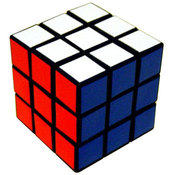
\includegraphics{cubefaces.jpg}
\caption{The solved cube}\label{cube}
\end{figure}


\begin{figure}[ht]
   \center
    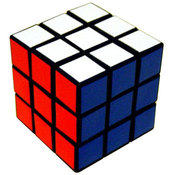
\includegraphics[scale=.5]{cubefaces.jpg}
\caption{A smaller solved cube}\label{cube2}
\end{figure}

\section{Bibliography}

Some sample books, web pages, and articles (from journals and conference 
proceedings) appear below in the reference section, which is generated using 
\bgn{thebibliography}\{{\tt N}\},
\nd{thebibliography}, 
where {\tt N} 
is the number of references.  (To be honest, 
{\tt N} can be any positive integer.  
For instance, in this file 
it is 3 while there are actually 4 references listed.)
If you want to cite a reference use 
\pln{cite}$\{${\tt name}$\}$ (not \pln{ref}$\{${\tt name}$\}$), 
like this: \pln{cite}$\{${\tt irros}$\}$ is \cite{irros}.  If you 
want to cite a page or specific result from a reference, you could do 
\cite[p.~340]{irros}, \cite[pp.~340--342]{irros}, or 
\cite[Theorem 20.1.1]{irros}. 
Place a tilde in the space between p. or pp. and the page 
numbers to prevent a line break in that space.  Take a look at the file 
to see how the citations were produced just above to know what this is about.

Here are two tips about typsetting references:

\begin{enumerate}

\item 
Be careful about how you type {\it left double quotes} and {\it right double quotes}.  
If you're not careful you get "this" instead of ``this''. See the LaTeX code for the previous sentence to learn how to make left quote marks appear correctly. 

\item
When a URL (webpage address) is in a reference, it is nice to color the URL blue so it's more apparent to a reader looking at your paper from a computer that clicking on the reference will bring up the webpage. Also, you  
may need a {\it twiddle} $\sim$ or an {\it underscore} \underline{ } in the URL.  You also may want to force a {\it linebreak} in the middle of the URL if it is too long to fit on one line of your output. Look in the code for typing \cite{gordina} to see how to achieve these effects with {\tt $\sim$gordina} and 
{\tt infinite\underline{ }Heisenberg}.

In particular, the URL is entered into the bibliographic entry twice: the first version is the actual URL, while the second version is what appears in your paper. You may use some LaTeX tricks for the {\it second} version to make it look nice, {\it e.g.}, a well-chosen space is used in 
\cite{gordina} to break the URL across two lines of the paper: {\tt gordina/infinite} is typed in the second version of the URL 
as {\tt gordina/ infinite} to force a line break at the term ``infinite''.


\end{enumerate}


\begin{thebibliography}{3}


\bibitem{gordina}
F. Baudoin, M. Gordina, and T. Melcher, Quasi-Invariance for Heat Kernel Measures on Sub-Riemannian Infinite-Dimensional Heisenberg Groups, 
{\color{blue}\href{http://www.math.uconn.edu/~gordina/infinite_Heisenberg_2011Full.pdf}{\tt http://www.math.uconn.edu/$\sim$gordina/ infinite\underline{ }Heisenberg\underline{ }2011Full.pdf}}.


\bibitem{irros}
K. Ireland and M. Rosen, ``A Classical Introduction to Modern 
Number Theory,'' 2nd ed., Springer-Verlag, New York, 1990.

\bibitem{joyner}
D. Joyner, ``Adventures in Group Theory'', 2nd ed., Johns Hopkins Univ. Press, 
Baltimore, 2008.

\bibitem{unabomber}
T. J. Kaczynski, Another proof of Wedderburn's theorem, 
{\it Amer. Math. Monthly} {\bf 71} (1964), 652--653.


\bibitem{roquette}
P. Roquette, Class field theory in characteristic $p$, its origin 
and development, pp.~549--631 in: ``Class field theory -- its centenary 
and prospect,'' Math. Soc. Japan, Tokyo, 2001.






\end{thebibliography}

\end{document}








